\documentclass[a4paper,10pt]{article}
\usepackage[T1]{fontenc}
\usepackage[utf8]{inputenc}
\usepackage{amsmath,mathrsfs,bm}
\usepackage{color}
\usepackage{cleveref}
\usepackage{graphicx}
\usepackage{fullpage}
\usepackage{natbib}
\newcommand{\jb}[1]{{\color{blue} (#1)} }
\newcommand{\gc}[1]{{\color{red} #1}}
\newcommand{\crefrangeconjunction}{--}
\begin{document}

\title{Convergence notes}

\author{
%Jeremy J. Berg$^{1,2}$, Joseph K. Pickrell$^{3}$, and Graham Coop$^{1,2}$ \\
$^1$ Center for Population Biology, University of California, Davis.\\
$^2$ Department of Evolution and Ecology, University of California, Davis\\
$^3$ New York Genome Center\\
\small To whom correspondence should be addressed: \texttt{jjberg@ucdavis.edu, gmcoop@ucdavis.edu}\\
}

\maketitle

Evolution (journal) has a commentary section, seems like something like that could work.

Why are we impressed by convergent evolution? Well it's because we get
to see selection act repeatedly to shape new mutations and standing
variation into adaptations in similar ways. This is particularly
impressive when we see convergence to a particular environment. Convergence helps us build
evidence that the phenotype is an adaptation, and form evidence that
adaptation is `for' increasing survival/fitness in particular
environment. 

How much do we say about genetic drift as a source of apparent convergence (and/or release from constraint).

Two distinct, but related questions, can we say that a phenotype/variant has been under selection. How many distinct instances of selection have there been. 
Related Q: as the more independent instances, the more evidence we have that it's
selected being selected.  

\paragraph{Formalizing the overlap in selection, in terms of selective
births/deaths}
When can we say that selection has been convergent in among populations?
Can we formalize this Q by thinking about the overlap in selective
deaths/births underlying the adaptative evolution of a particular trait, allele, or set of alleles within a population?

One locus:\\
The selective load (L) for directional selection (where fitest homozy
has selection coeff $s$) move an allele from frequency $x_1$ to $x_2$
in $t_1$ to $t_2$ generations is
\begin{align}
L &= \sum_{t=t_1}^{t_2} s(1-x_t) \\
&\approx \int_{t_1}^{t_2}  s(1-x_t) dt
\end{align}
The number of selective deaths, in a population size of $N$, is
$NL$. Assuming an additive model ($dx/dt = (s/2)x(1-x)$) 
\begin{align}
L &= \int_{t_1}^{t_2}  s(1-x_t) dt\\
&= 2  \int_{x_1}^{x_2}  \frac{1}{x} dx\\
& = 2 \log(x_2/x_1) 
\end{align}
So if the ancestral population goes from frequency $x_1$ to $x_2$, and
the descendant populations ($1$ and $2$) move this to $x_3^{(1)}$ and
$x_3^{(2)}$, then their shared deaths are $2N\log(x_2/x_1)$ and separate
deaths are $2N\log(x_3^{(1)}/x_2)$ and
$2N\log(x_3^{(2)}/x_2)$. The fraction of shared deaths would be ratio
\begin{equation}
\frac{\log(x_2/x_1)}{\log(x_3^{1}/x_1)}~~~\textrm{and}~~~\frac{\log(x_2/x_1)}{\log(x_3^{1}/x_1)}
\end{equation}
Interestingly this is mostly determined by deaths when the
allele when it is rare (wonder if this means HH will be informative).\\

Phenotype:\\
The response to selection, for a phenotype with heritability $h^2$ and
phenotypic variance $V_p$, is 
\begin{align}
R = h^2 i(p) \sqrt{V_p}
\end{align}
where $i(p)=S/sqrt{V_p}$, $i(p)$ is the selection intensity. So if the
population achieves a phenotype shift $R_T$ in $T$ generations, then
the implied selection intensity per generation is 
\begin{equation}
i(p) = \frac{R_T}{h^2 T \sqrt{V_p}}
\end{equation}  
Under trunctation selection (Lande says it the form of selection that
implies weakest selection) we can obtain the fraction ($p$) of individuals
who were parents from $i(p)$, but this isnt a nice simple
expression. Perhaps just talking about fraction of phenotypic change would be
enough, and point out that this is linked to the intensity of
selection. 

\paragraph{Why is this easier when we have changes polarized on a phylogeny?}

Why is this question easier when we have a resolved phylogeny with
no-incomplete lineage sorting.
Well in that case the selective births and deaths are clearly
independent. E.g. the individuals who lived/died, due to differential
predation pressure, to drive the adaptation of light coloured fur in
arctic foxes and hares were clearly different sets of individuals
(being foxes and hares respectively). 

%Useful bib of convergence
%http://www.oxfordbibliographies.com/view/document/obo-9780199941728/obo-9780199941728-0038.xml

If we have a tree of drift (w. no gene flow), seeing non-sisters sharing an selective
event can be ``enough''. E.g. if both populations show a sweep (A \& C), not
shared with sisters (B \& D), then we have evidence that selection has occurred
in both pops independently. 

\paragraph{What do we mean, or can we say about, convergence when we only see the selected allele}


\begin{figure}
	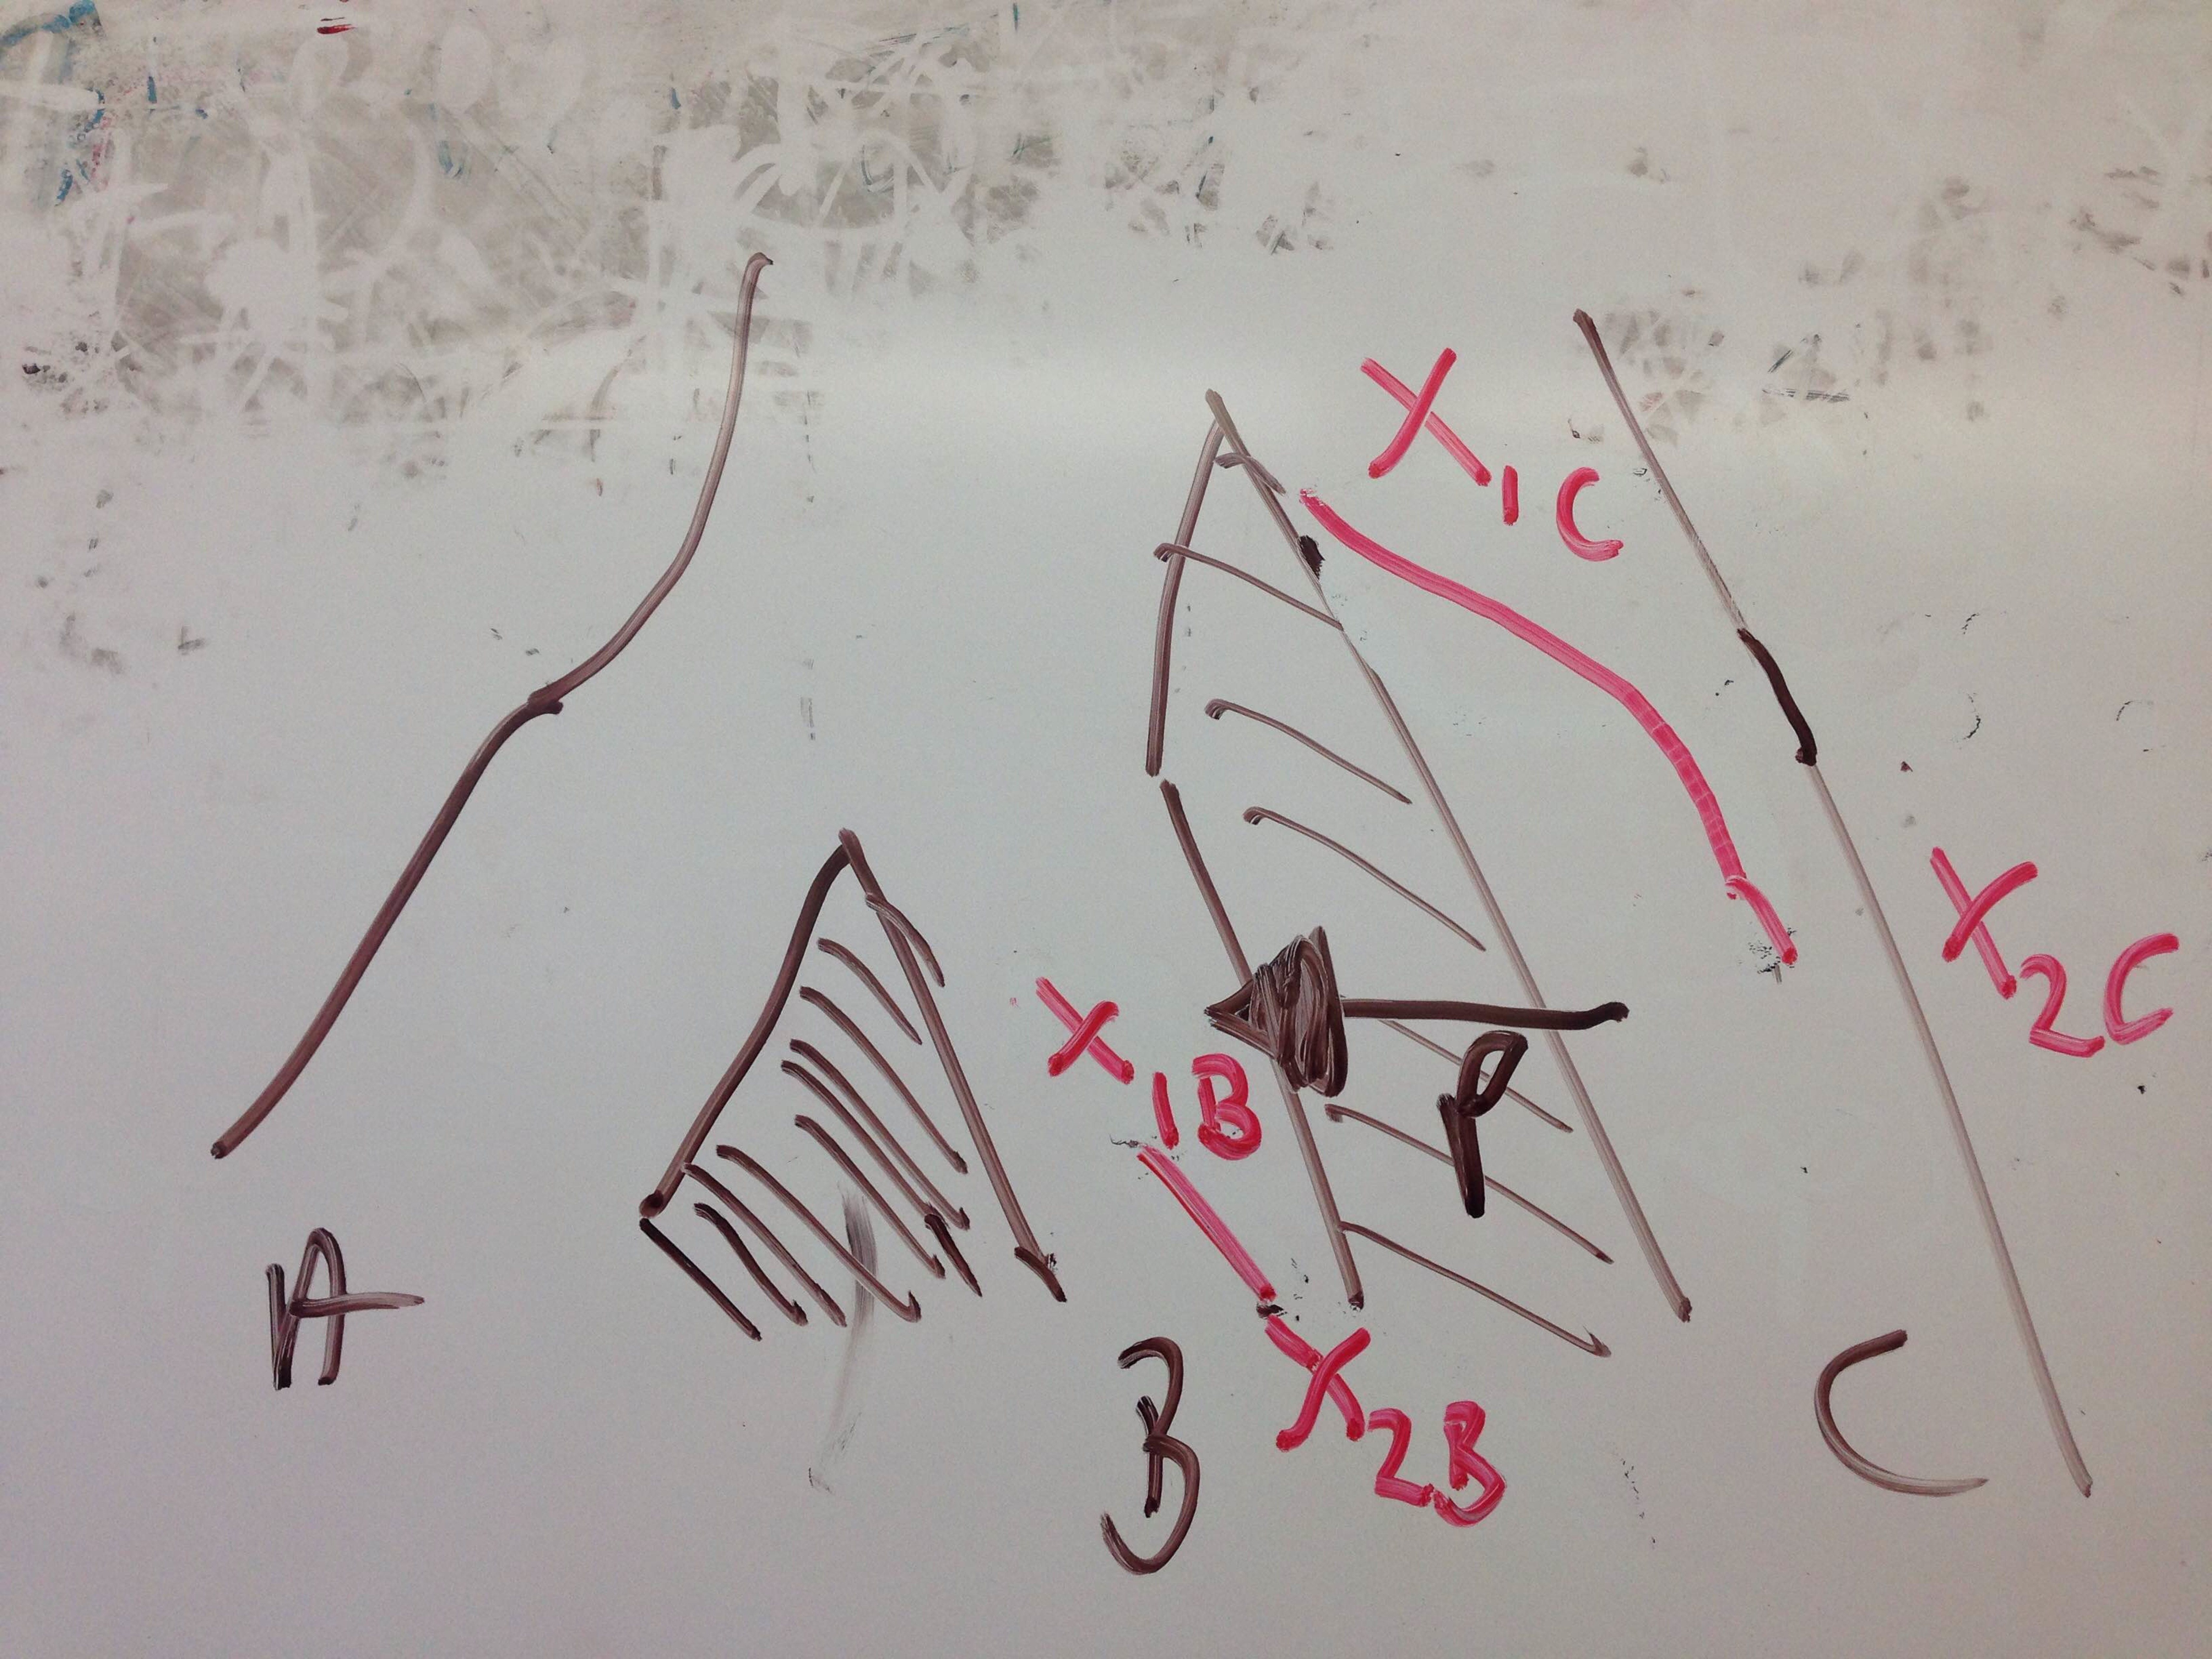
\includegraphics[width = 0.4\textwidth]{Figures/single_allele_admixture}
	\caption{BLAH}
	\label{fig:admix-graph}
\end{figure}
Consider the case, showin in Figure \ref{fig:admix-graph}. The selected allele has changed frequency in
population C, and there is gene flow from C into B (w. admixture
prop. $p$), but not into $A$. The question is, is how much convergence
has occurred in popualtion $B$?  
Assume first that allele is absent in
$A$ and was absent in $B$ prior to admixture.  The change in $C$ is
from $x_{1C}$ to $x_{2C}$. Assume that
$x_{2C}$ was the frequency when admixture occurred, an assumption conservative
against finding convergence. Then $x_{1B}$, the frequency immediately
following admixture is $pX_{2C}$. Then the selective deaths in
population $C$ and $B$ are
\begin{equation} 
2N\log(x_{2C}/x_{1C})~~~\textrm{and}~~~2N\log(x_{2B}/px_{2C})
\end{equation}
So most of the selective death will have been in population $C$ when
$px_{2C} \gg x_{1C}$. I.e. most of the action is getting the allele to
appreciable frequency, the selection after admixture is minor if the
admixture prop. is not low.\\ 

Seems like there's two questions: how much of
the selective death is shared? Is there evidence of selection at all
in population $B$ or is drift and admixture sufficient to explain the
frequency of the allele in population $B$, with selection only occurs
in population $C$.

\paragraph{What do we mean, or can we say about, convergence when we see the linked variation/sweep?}

\paragraph{What do we mean by convergence when we are thinking of quantitative traits?}
Should we also cover when phenotypes alone are seen? in that case using covar matrix can help in QST style analysis.
Idea of double sign test?



\paragraph{Issues about meaning of convergence when there is incomplete lineage sorting} 
%http://www.indiana.edu/~hahnlab/Publications/HahnNakhleh2016.pdf


\paragraph{Long term signal?}
Can long term selection/drift on trait or variant, erode signal of shared
history. E.g. id stabilizing selection acts separately on a shared
trait in two (now independent populations) can we fix alternate
solutions, even though we original shared pool. Similar Q about shared
haplotypes whittled away by recom/migration. 
--One Q is do we care? 


\end{document}